\section{Low Threshold Cherenkov Counter}


\subsection{Geometry}
The LTCC mirror geometry is implemented through the native gemc geometry API. The elliptical mirrors are made through a subtraction of
two G4Ellipsoid. The hyperbolic mirror are built using geant4 polycon approximating the mathematical shape using about 30 segments.
The cylindrical mirrors are made of G4Tubs.

The LTCC winston cones are of three types: small, medium and large. Three CAD models are tessellated and imported in the simulation, and
then are copied into 36 WC / sectors using the perl api.

Finally, the LTCC Box, mirror support structure and additional support hardware are imported directly from the engineering CAD models.
The \F{ltccGeometry} shows details of the geometry implementation.

\begin{figure}
	\centering
	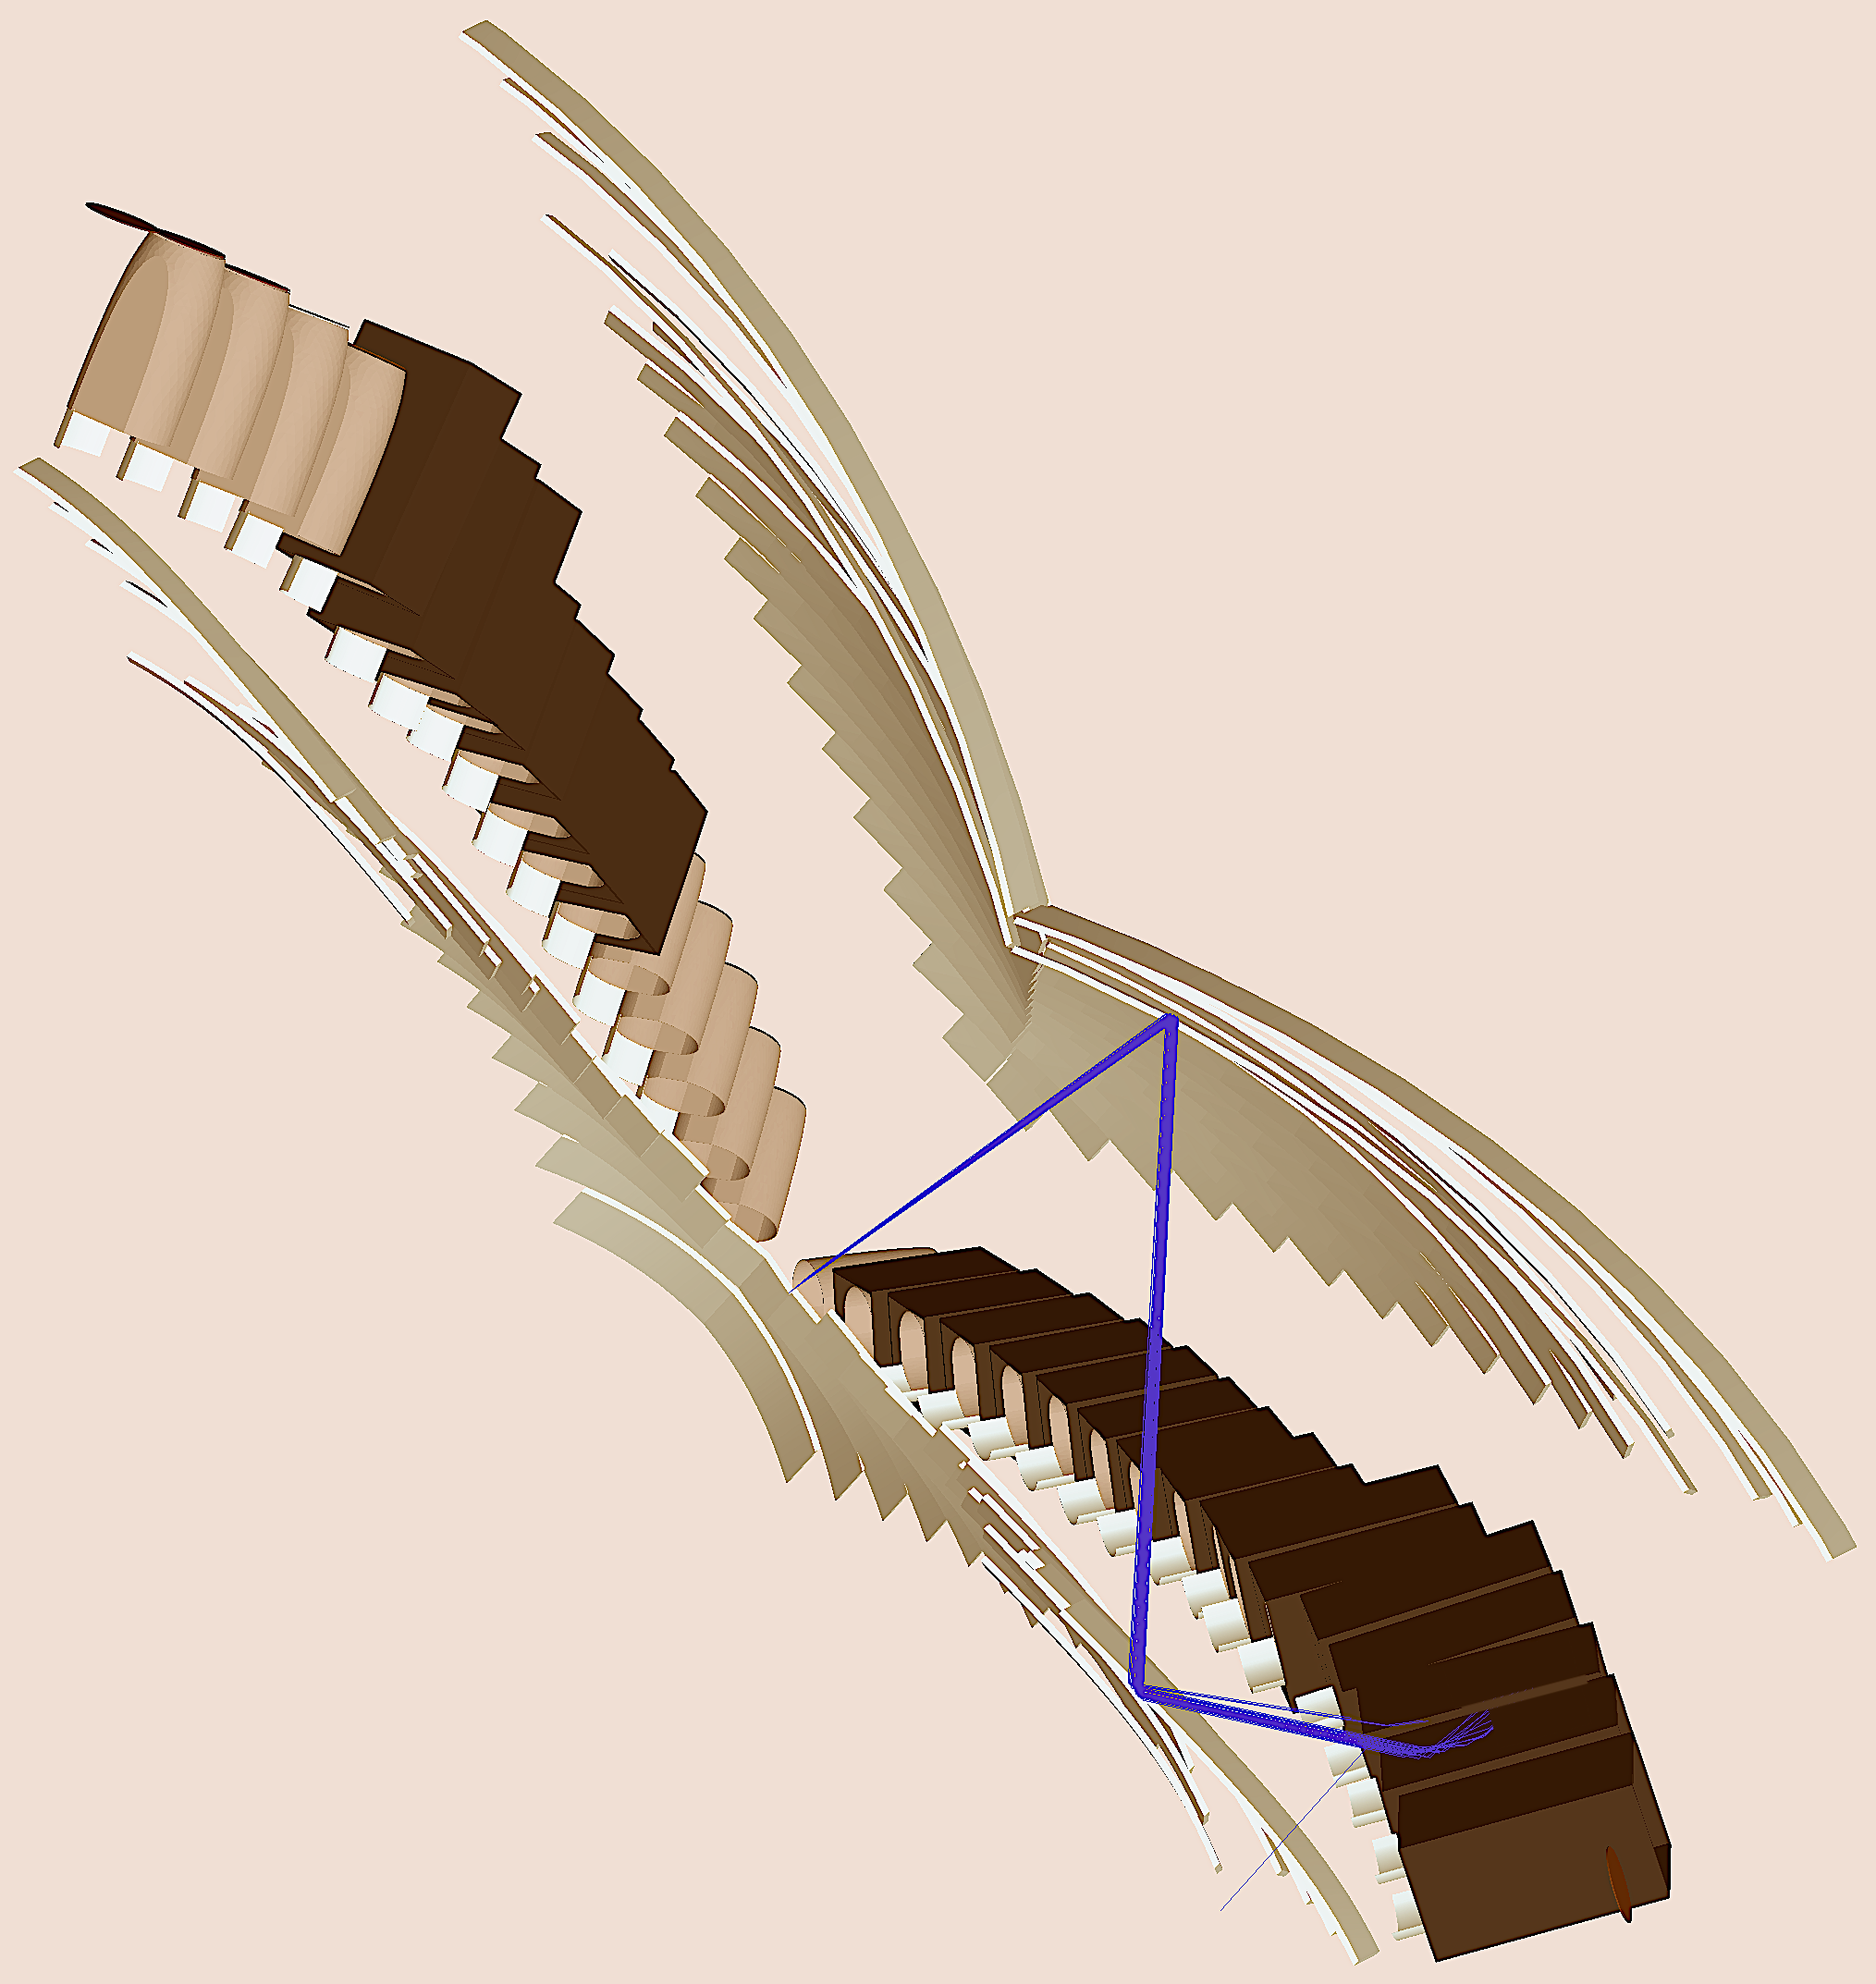
\includegraphics[width=0.95\columnwidth,keepaspectratio]{img/ltccGeometry.png}
	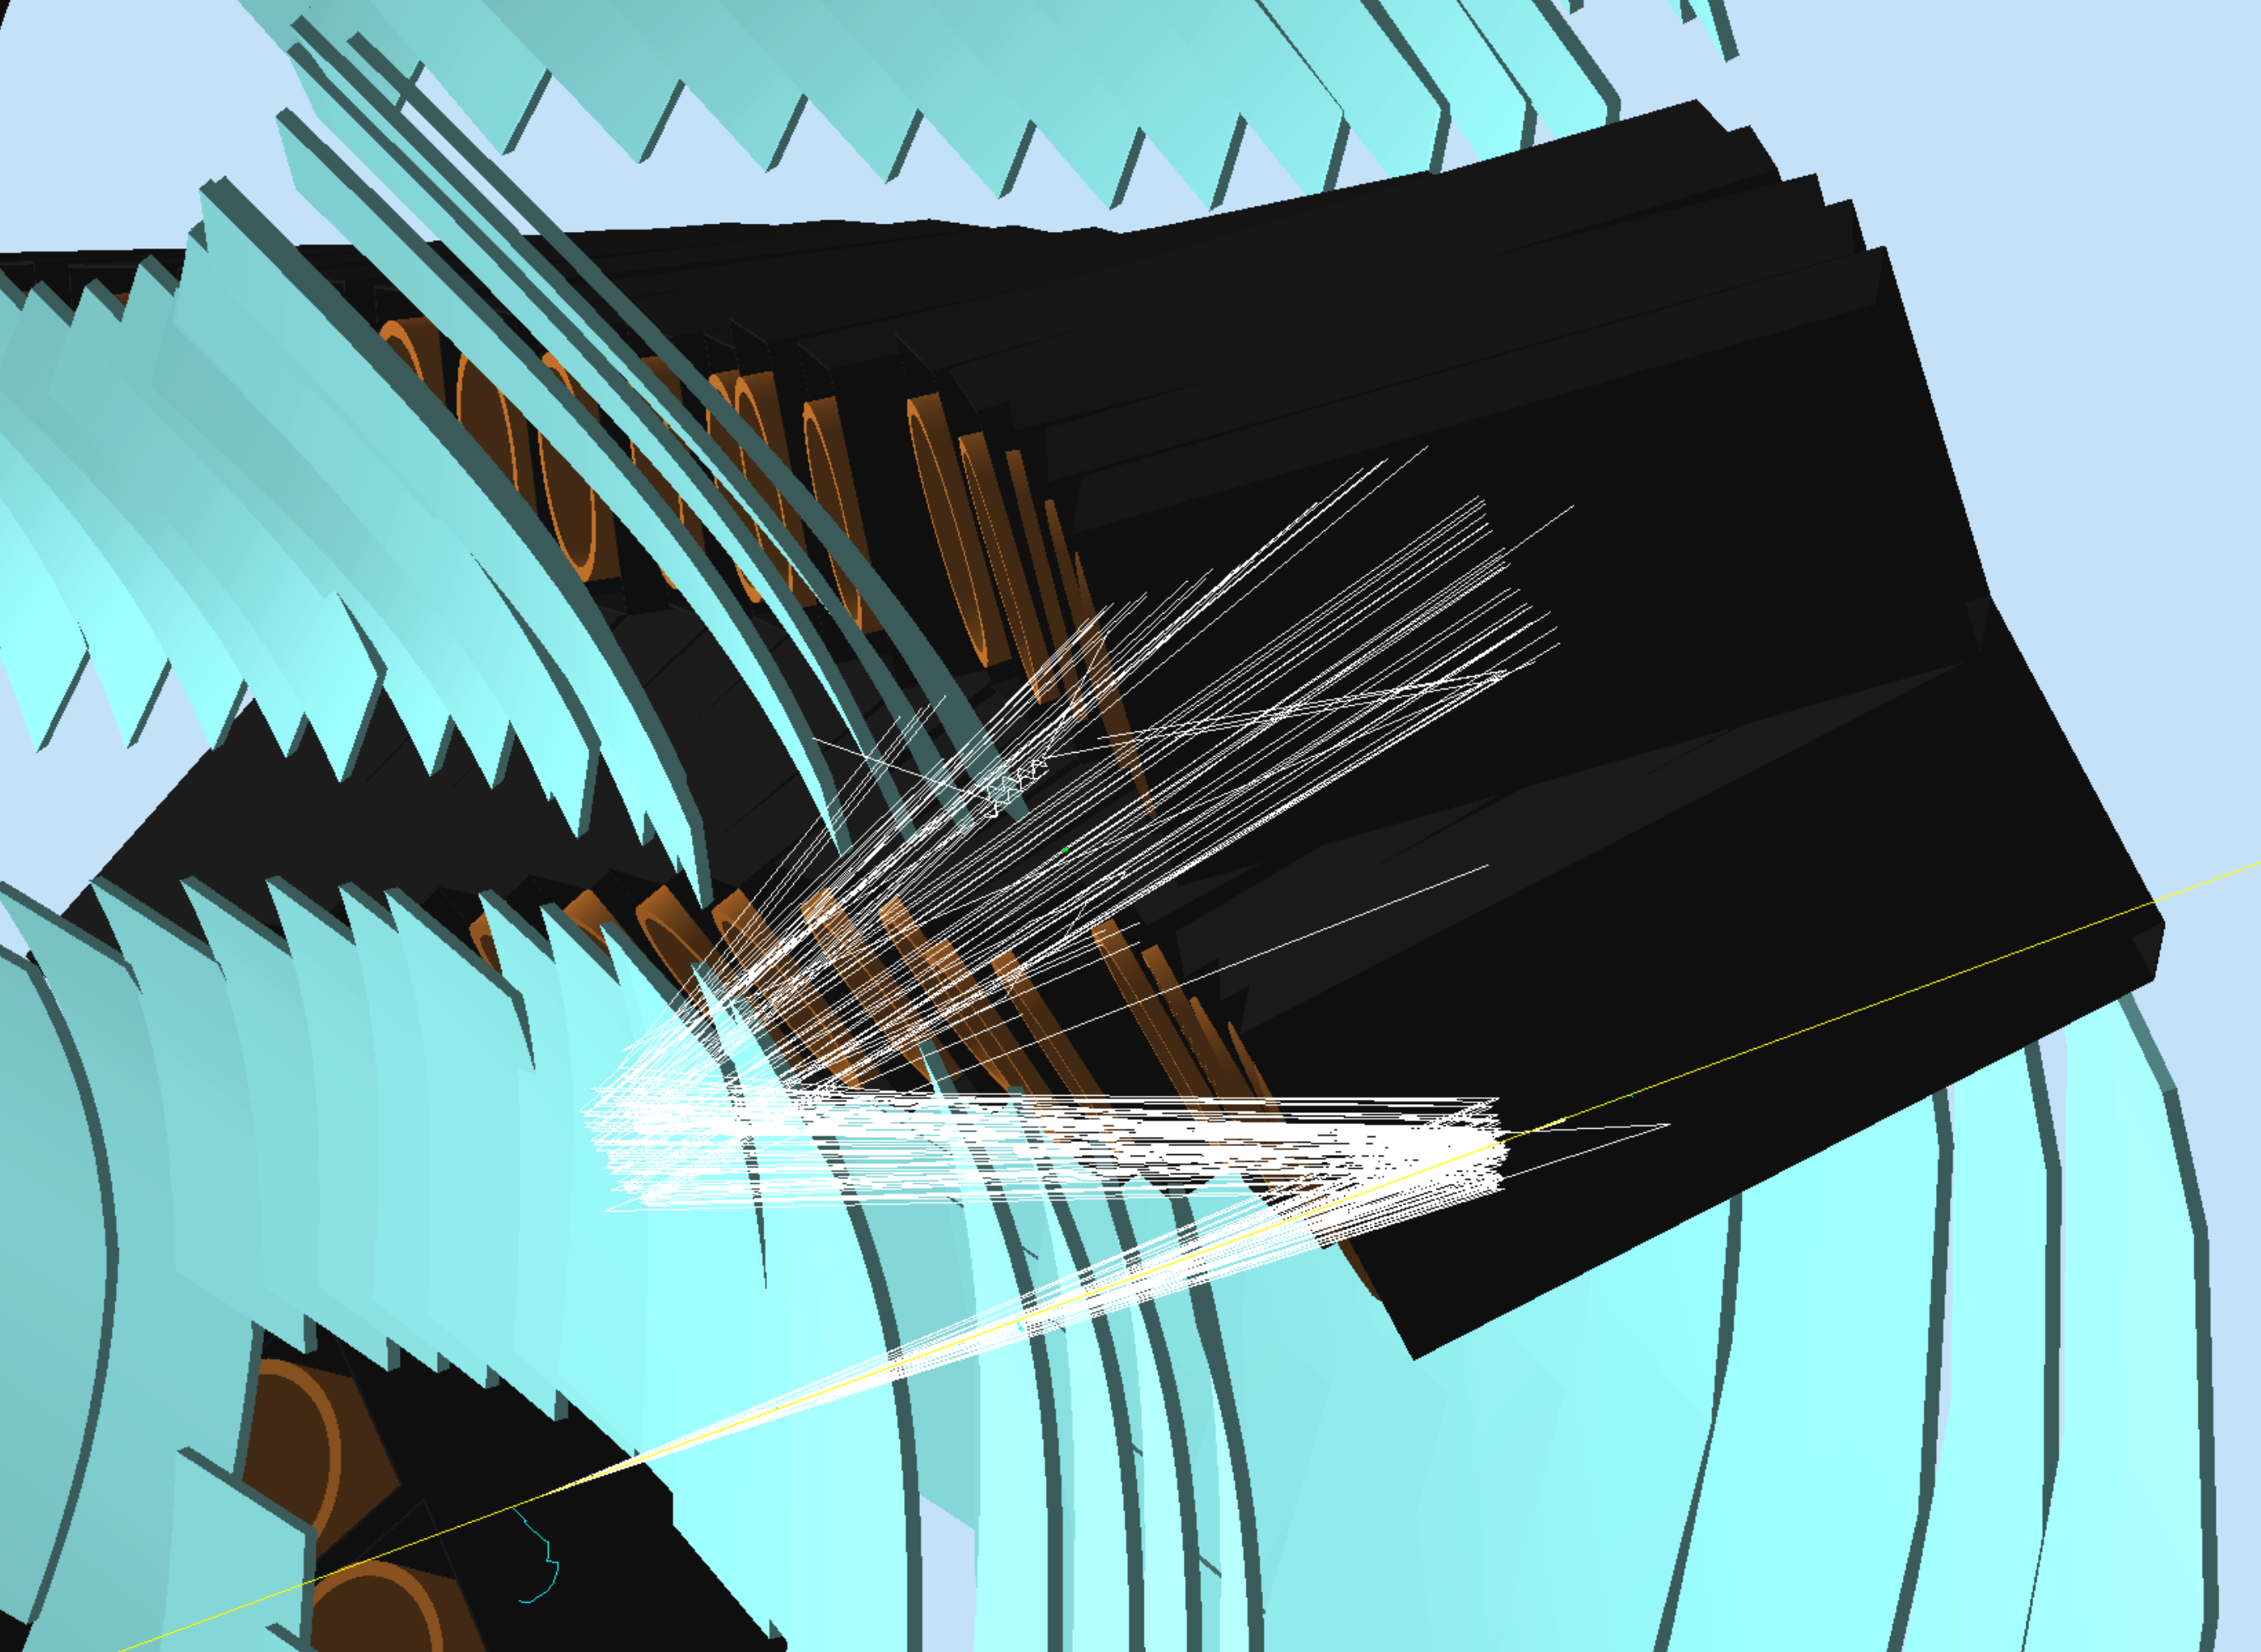
\includegraphics[width=0.95\columnwidth,keepaspectratio]{img/ltccDetail.png}
	\caption{Top: the GEMC implementation of the EC geometry. The paddles are G4Boxes, embedded in trapezoid representing the mother volumes of each panel.
            Bottom: a zoom-in of the implementation shows the details of the individual paddles for Panel 1B (green) and Panel 1A (purple) }
	\label{fig:ecGeometry}
\end{figure}

The refractive index of the $C_4F_10$ and its transparency is included in the material optical properties and taken
into account during the geant4 transportation of the phtotons.

The mirror and winston cones reflectivities are associated with the mirror optical properties and are taken into
account and taken into account during the geant4 transportation of the phtotons.

The quartz window PMT quantum efficiency are associated with the PMT face optical properties and are taken into account in
the digitization routine.

\subsubsection{Geometry Git Location}
The github location of the gemc perl api script is  \url{https://github.com/gemc/detectors/tree/master/clas12/ltcc}.


\subsection{Digitization}

Photons that impinged on the PMT faces are processed with the digitization routine.
For each photon collected undergoes the quantum efficiency algorithm at its wavelength to decided if it's finally detected.
The adc is calculated and smeared using the single photo-electron peak position and sigma from the calibration database.


\subsubsection{Timing}

The time average of all the photons is saved in the output.

\subsubsection{Summary of CCDB Table used}

\begin{itemize}
	\item /calibration/ltcc/spe
\end{itemize}

\subsection{Digitized Bank}

The digitized output bank has $ID=1400$, and the variables are summarized in Table \ref{tab:ltccBank}

\begin{table}
	\begin{center}
		\begin{tabular}{| c | c | c |}
			\hline \hline
			Variable    & Description                                        & Tag  \\
			\hline
             sector  &                                     clas12 sector  &    1 \\
               side  &                               left or right index  &    2 \\
            segment  &                                           segment  &    3 \\
                adc  &                                               adc  &    4 \\
               time  &                           average time of the hit  &    5 \\
               nphe  &                  number of photoelectrons arrived  &    6 \\
              npheD  &                 number of photoelectrons detected  &    7 \\
               hitn  &                                        hit number  &   99 \\
			\hline \hline
		\end{tabular}
	\end{center}
	\caption{The digitized LTCC bank}\label{tab:ltccBank}
\end{table}

\subsubsection{Time Window}
The timewindow of the LTCC is set to 5 ns.


\subsubsection{Background merging algorithm}

\subsubsection{Process Routine Git Repository Location}
The LTCC hit process routine location in git is \url{https://github.com/gemc/source/blob/master/hitprocess/clas12/ltcc_hitprocess.cc}
